\newpage
\setcounter{page}{1}
\justifying
\noindent

\section{Introduction}
\subsection{Formula Student}
Formula student United Kingdom (FSUK) is an annual motor-sport engineering competition which held by Institute of Mechanical Engineers (IMechE). Formula student was first run by its inception, The Society of Automotive Engineers (SAE) in 1981 in the United States of America which known as Formula SAE. Every July since 2007, hundreds of universities from around the world gather at Silverstone Circuit for the final competition. The objective of every team is to design and build a single-seat race car which then will be judged from number of engineering and business aspects.

\noindent The competition mainly consist of 2 events: static and dynamics. The static event judges the Engineering  Design,  Cost  and  Sustainability  Analysis, Business Presentation and Technical Inspection, and the dynamic event judges Skid Pad, Sprint, Acceleration, Endurance, and Fuel Economy.


\begin{figure}[!ht]
\begin{center}
%    
  \begin{subfigure}[b]{0.4\textwidth}
    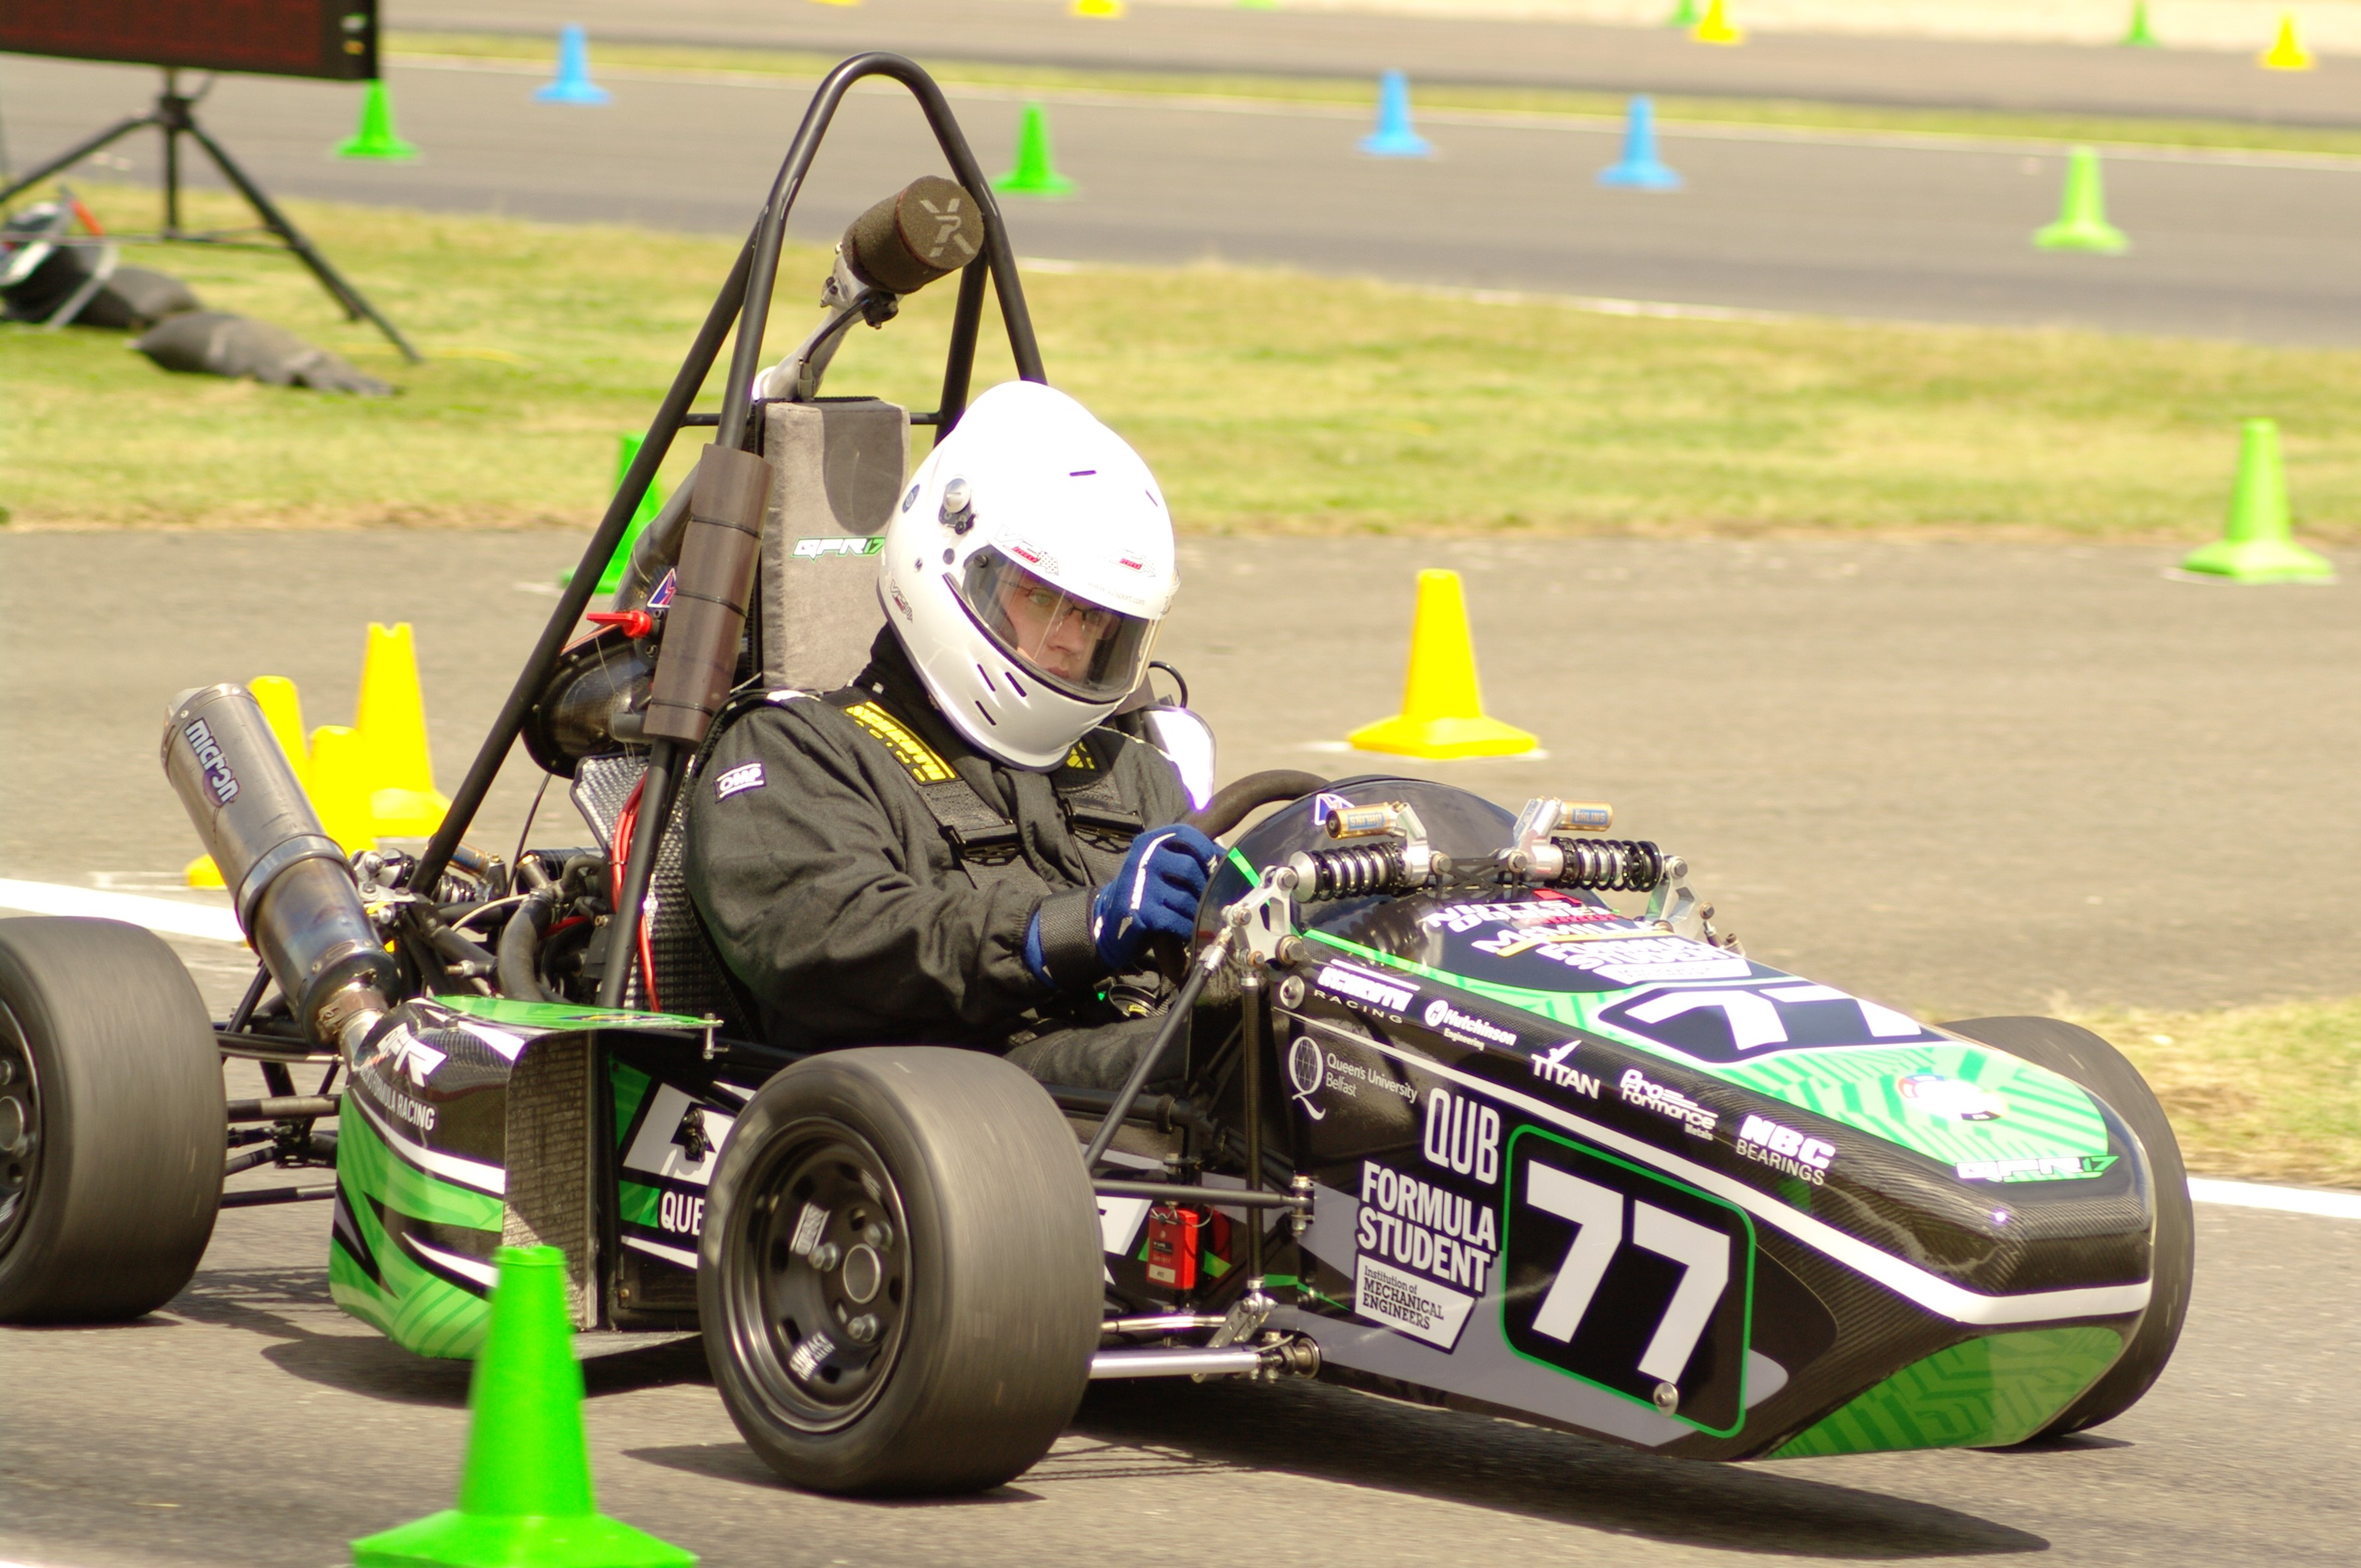
\includegraphics[scale=0.05]{Figures/QFR17PHOTO.JPG}
  \end{subfigure}
  %
  \begin{subfigure}[b]{0.4\textwidth}
    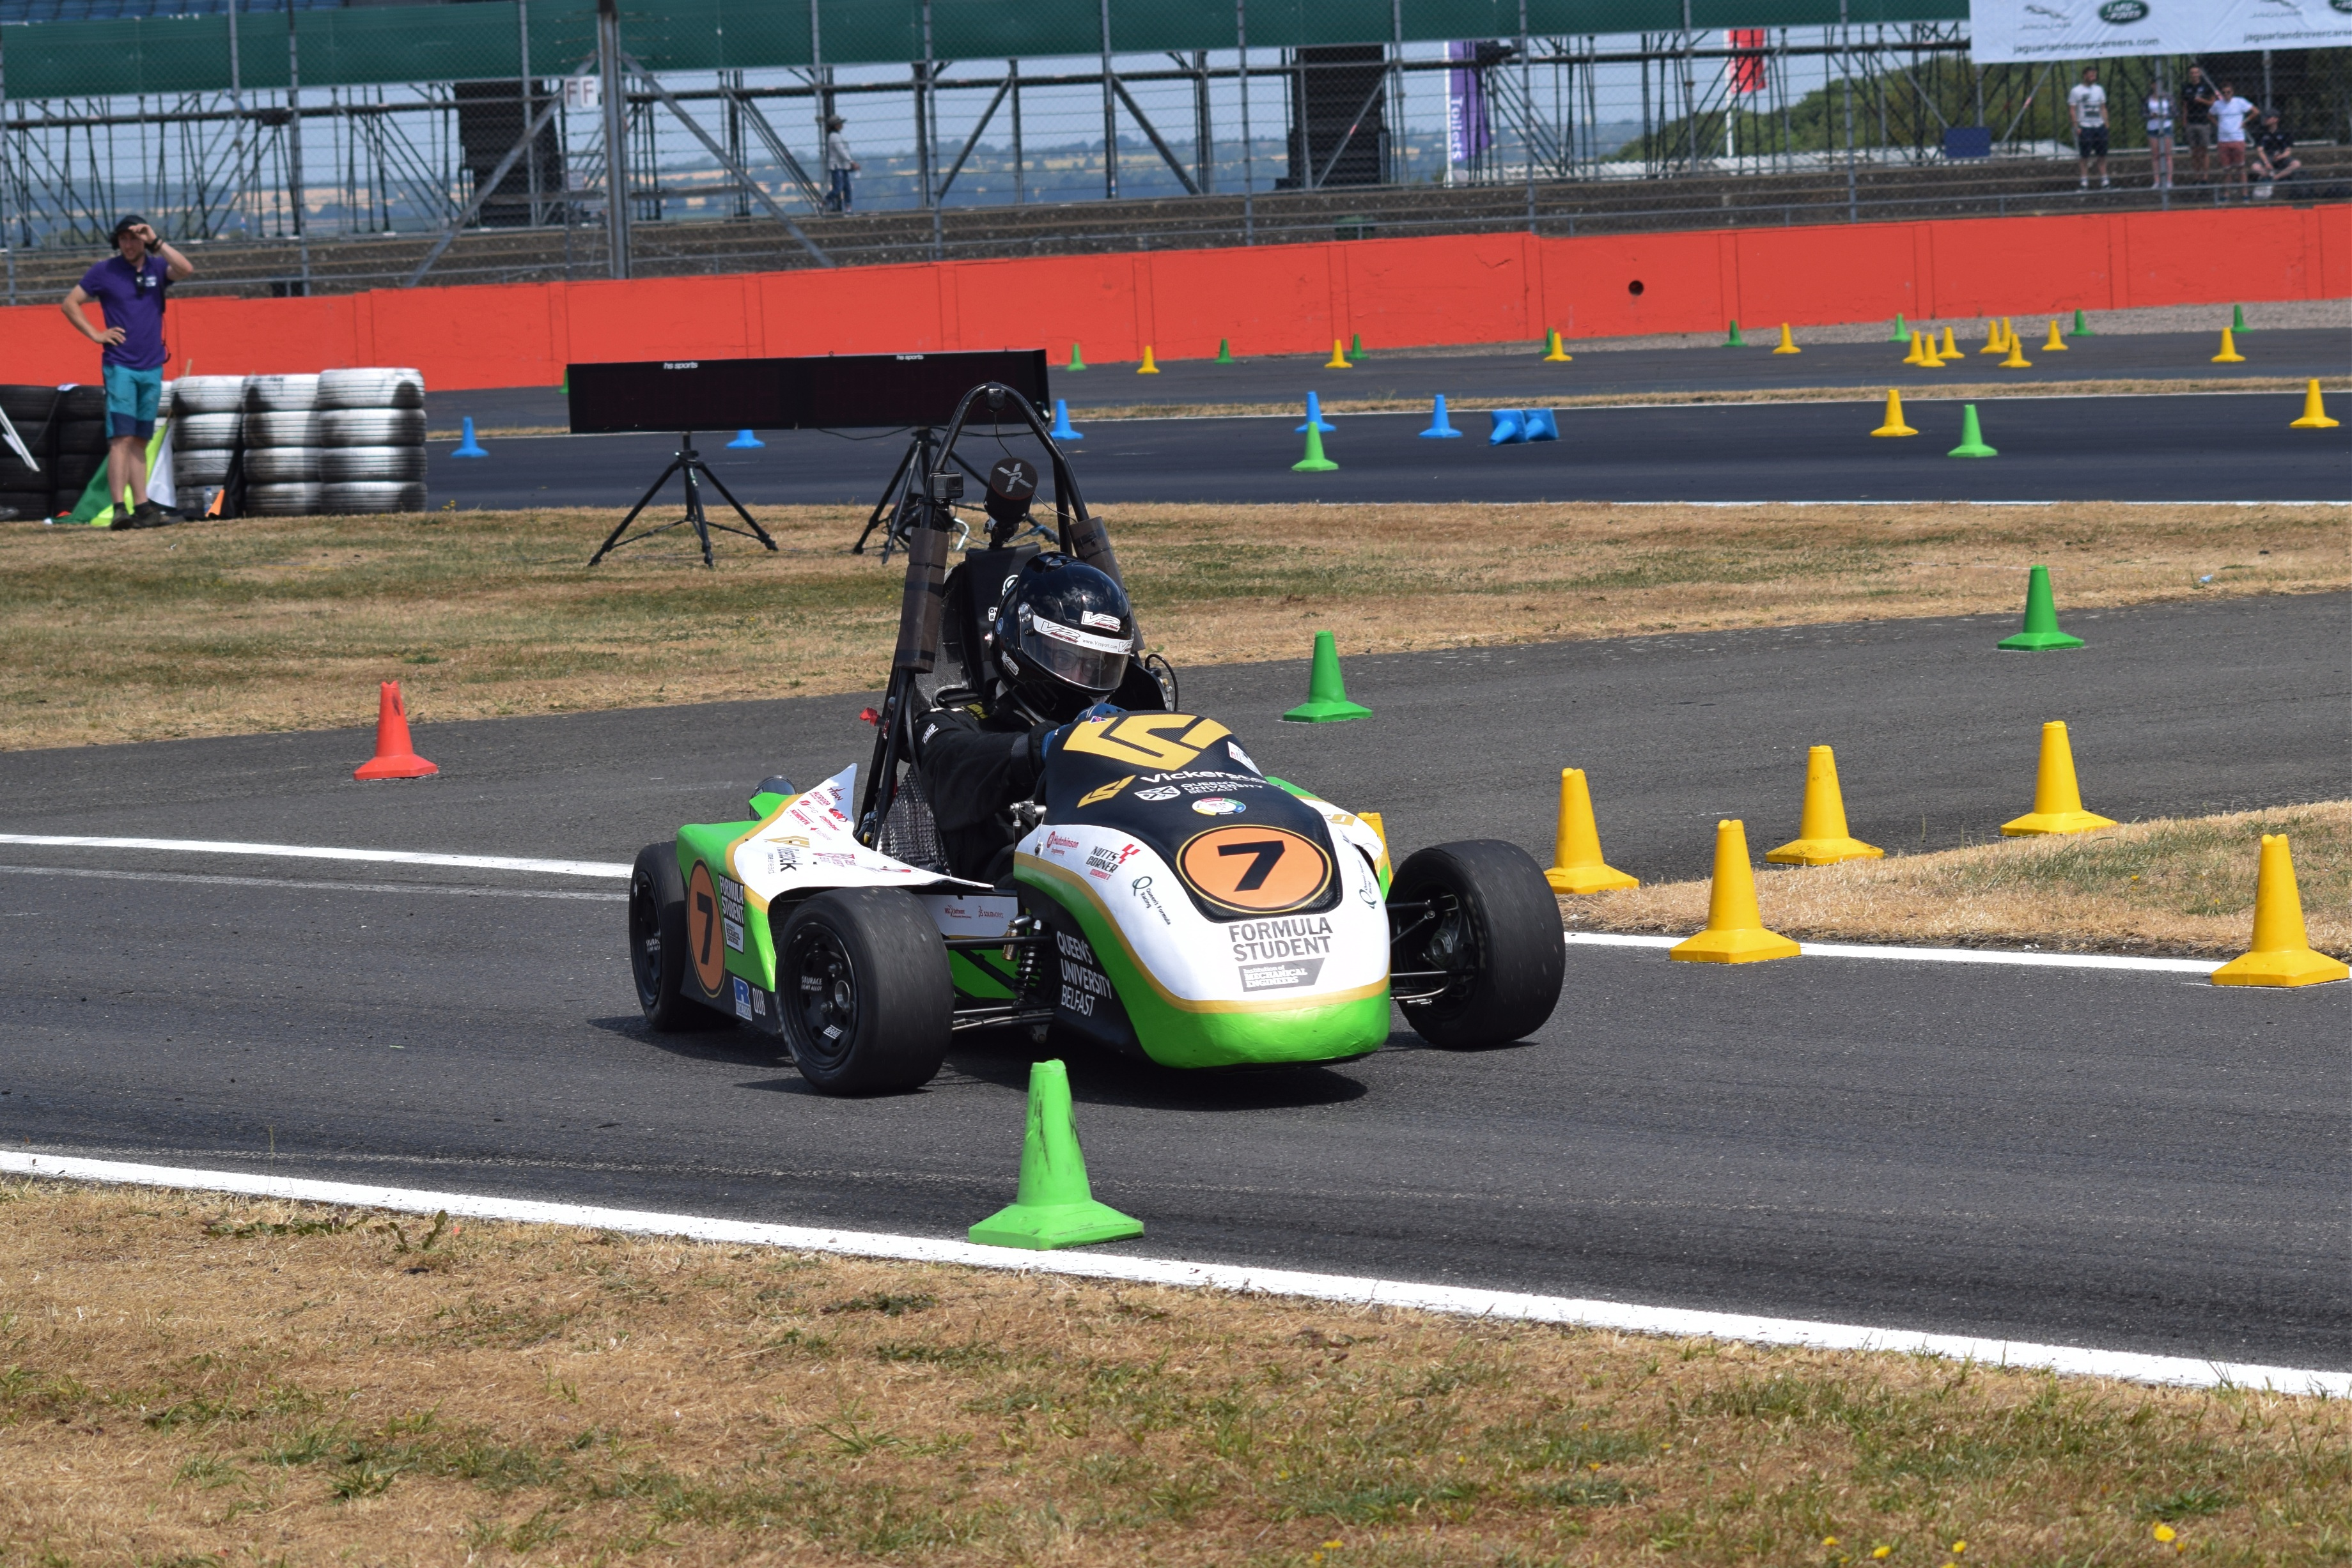
\includegraphics[scale=0.05]{Figures/QFR18PHOTO.jpg}
  \end{subfigure}
%  
  \caption{Queen's Formula Racing car 2017(left) and 2018 (right) on the dynamics event}
    \label{fig:1}
\end{center}
\end{figure}


\noindent Queen's University Belfast is represented by Queen's Formula Racing (QFR) in the event of FSUK since 2007. The team is consisted of undergraduates and postgraduate students which are divided into Engineering sub-teams focusing on chassis, suspension \& unsprung mass, powertrain, electrical, and performance. Consideration of aerodynamic aspect on QFR car was first initiated in 2017 which focus on the aerodynamic analysis framework\cite{Corr2017MechanicalAuthor}. In 2018 the first design of aerodynamics undertray for QFR race car was generated\cite{McKeown2018DesignCar}, and this paper is intended to build up the analyses from previous paper and improve the undertray performance by investigating broader and deeper to the variables which could plausibly enhance the overall car performance.  

\subsection{The significance of Aerodynamics in Formula Industry}
Aerodynamics has become a crucial aspect to the high-speed cars performance. The race-car industry has led the technology innovation by indicating the needs of constant improvements \cite{Zhang2006GroundCars}. Engineers have been trying to modify the car's shape to manipulate and advantages the flow around the body. The role of aerodynamics in improving the race-car performance rose in 1968 when inverted airfoil was introduced to Formula One car, and the research in this area has been growing exponentially ever since. 

%put inverted aerofoil race car photo here

\noindent Downforce(negative-lift) is one of the major aerodynamics key in improving the overall race-car's performance. Downforce or negative lift is force product of the aerodynamics flow around the body. On high-speed ground vehicle, this usually achieved by introducing aerodynamic devices such as wing (inverted wing) and undertray which modify the airflow to the engineering needs \cite{Wright1982TheCars}. In the race-car industry, the primary aim is to maximise the downforce while maintaining the drag at the lowest \cite{Zhang2006GroundCars}, but achieving constant performance at diverse speed and acceleration is equally important.  The size of downforce is significantly affected the breaking acceleration and cornering, hence the cornering speed. Despite the restrictive aerodynamics rules in the competition, optimising the downforce could potentially improve the acceleration which increases the chance to overturn the opponent on a corner. Higher downforce could also increase the top-speed in shorter time that reduces the corner entry and exit time. A ground effect aerodynamics that applied to an open-wheeled car is still an experimental science \cite{Zhang2006GroundCars}, this is due to the complex physics flow that involve turbulent wake, interaction of ground boundary layer, dynamic suspension motion, and many more in which accurate analytical capability (experimental \& computational) is not yet sufficient.

\noindent Nevertheless, computational fluid dynamics (CFD) has improve tremendously with the industry over the years and able to produce an accurate results of forces, flow pattern, etc, in some particular geometry of the car. However, one research paper \cite{Zhang2006GroundCars} stated that diffuser is one part of race car that can be hardly understood, therefore specific variable in generating an undertray geometry is required with careful consideration and assumption on the analysis. 

\noindent In this paper, computational fluid dynamics will be used to understand the trend behaviour of an aerodynamics undertray in 2 dimension and 3 dimension with numbers of nozzle \& diffuser variables such as angle, length, and width. These results then will be used as consideration for the geometry dimension of the final aerodynamics undertray for QFR 2021.

\subsection{Project Aims \& Objectives}
The aim of this project is to design and optimise the aerodynamics undertray for Queen's Formula Racing car which improve the car's overall down-force and drag reduction. Final design of the undertray will be based on the computational simulations and design recommendation from previous QFR analysis. The approved final design then will be manufactured and installed to QFR 2021 for the competition if the workshop time and capacity allows.

\noindent
To fulfill the project aim, there were some objectives made:
\begin{itemize}
    \item Analyse the enclosed and open flow 2D \& 3D analyses with various inlet, outlet, and ground clearance variables  using ANSYS Fluent to identify its effect and trend on the undertray lift and drag. 
    \item Design flexible 3D undertray designs based on the 2D analysis results, which then will again be optimised with additional aerodynamic features on the undertray which will improve the downforce and reduce the drag.
	\item Design the final undertray CAD and choose the material which tailored to car’s dimension and goals, then analyse the weight to drag ratio to pick the best performance and material for the car
    \item Manufacture and fit the undertray for 2021 Queen’s Formula Racing car which then will be judged on the Formula Student competition.
\end{itemize}